
\section{Diagramas de Flujo}
A continuación se describen en detalle los procesos principales del sistema,
trazando el recorrido de cada comando desde la entrada en la CLI hasta la
respuesta final al usuario. El sistema expone veinte comandos operativos que
se pueden agrupar en seis familias funcionales: gestión de usuarios, gestión
de capital, obtención de datos, gestión de estrategias, inteligencia artificial
y consultas informativas.

% =============================================================================
\subsection{Gestión de Usuarios y Acceso}
% =============================================================================

La Figura~\ref{fig:login} muestra el flujo de entrada principal del usuario
a través de la interfaz de línea de comandos (CLI), incluyendo autenticación,
registro y ayuda. El \textit{dispatcher} principal de la CLI intercepta la
línea introducida y la enruta al comando correspondiente mediante el registro
de comandos inicializado al arrancar la aplicación. Todos los comandos
operativos verifican en primer lugar que exista una sesión activa antes de
ejecutar cualquier lógica; los comandos de autenticación, en cambio,
comprueban lo contrario: que el usuario no haya iniciado ya sesión.

\textbf{Flujo de registro (\texttt{signup}).}
El comando solicita nombre de usuario y contraseña de forma interactiva.
El caso de uso de creación de usuario comprueba, dentro de una transacción de
solo lectura, que no exista otro usuario activo con ese nombre en la base de
datos. Si el nombre está libre, la contraseña se transforma con BCrypt antes
de que el objeto usuario sea persistido: la contraseña en claro nunca se
almacena ni se transmite a la capa de persistencia. Si el nombre ya existe,
el sistema lo notifica al usuario y el registro no se completa. Esta decisión
de validar unicidad por nombre de usuario (en lugar de por correo electrónico)
simplifica el flujo de registro y la experiencia en la CLI, donde no hay
formulario web que facilite la entrada de texto largo.

\textbf{Flujo de autenticación (\texttt{login}).}
El comando solicita nombre de usuario y contraseña. El caso de uso de
autenticación recupera el hash almacenado para ese nombre y lo coteja con la
contraseña proporcionada usando BCrypt de Spring Security Crypto. Si la
verificación es positiva, el gestor de sesión registra el usuario en la
variable de sesión de la aplicación, habilitando todos los comandos
operativos. Si las credenciales son incorrectas, el sistema notifica el fallo
sin especificar qué campo falló, evitando revelar si el nombre de usuario
existe en la base de datos. Al apagar la aplicación, el gestor de sesión
detecta el cierre del contexto de Spring y liquida todas las estrategias
activas antes de que el proceso termine, garantizando que ningún proceso
Python quede huérfano.

\begin{figure}[H]
    \centering
    
\includegraphics[width=0.9\linewidth]{Fotos/diagramas-flujo/inicio-registro-ayuda.png}
    \caption{Flujo de autenticación (login/signup) y ayuda}
    \label{fig:login}
\end{figure}

% =============================================================================
\subsection{Gestión de Capital (\textit{Wallets})}
% =============================================================================

La Figura~\ref{fig:wallets} muestra el proceso de creación y consulta de
billeteras virtuales. La plataforma soporta billeteras de tipo papel
(\textit{paper trading}) para operar con capital simulado, y el ciclo de vida
de cada billetera está estrechamente ligado al del libro mayor contable
(\textit{ledger}), que registra cronológicamente todos los movimientos de
capital.

\textbf{Listado de billeteras (\texttt{lw}).}
El comando verifica que haya sesión activa y delega en el servicio de gestión
de billeteras, que consulta todas las billeteras asociadas al identificador del
usuario en sesión, ordenadas por nombre. Para cada
billetera se muestra el saldo real (\textit{equity} acumulado incluido PnL
realizado), el saldo disponible para nuevas operaciones y un indicador
\texttt{[EN USO]} cuando la billetera tiene estrategias activas. Esta
distinción entre saldo real y saldo disponible es fundamental: el saldo
disponible se reduce en el momento en que se activa una estrategia y no se
recupera hasta que ésta se liquida definitivamente, aunque se pause en medio.

\textbf{Creación de billetera (\texttt{mkpwallet}).}
El comando solicita nombre y saldo inicial. El servicio de gestión de
billeteras comprueba que no exista ya una billetera con ese nombre para el
usuario actual. Si el nombre está disponible y el saldo es positivo, se crea
la billetera con saldo real y saldo disponible iguales al depósito inicial y
tipo \texttt{WalletType.PAPER}. La billetera queda en estado inactivo hasta
que se asigne a una estrategia. Cuando una estrategia se activa, el servicio
contable adquiere un bloqueo pesimista sobre la billetera y sobre la propia
instancia de estrategia antes de restar el capital del saldo disponible;
este mecanismo previene condiciones de carrera en escenarios de concurrencia
en los que varias estrategias pudieran activarse simultáneamente sobre la
misma billetera. En ese mismo instante se registra en el libro mayor una
entrada de tipo \texttt{RESERVED} con importe negativo, garantizando la
trazabilidad completa de cada movimiento de fondos desde el depósito inicial
hasta la liquidación final.

\begin{figure}[H]
    \centering
    
\includegraphics[width=0.7\linewidth]{Fotos/diagramas-flujo/creacion-listado-wallets.png}
    \caption{Proceso de creación y listado de \textit{wallets}}
    \label{fig:wallets}
\end{figure}

% =============================================================================
\subsection{Obtención de Datos (ETL)}
% =============================================================================

El comando de descarga implementa un mecanismo incremental que minimiza las
peticiones a la API de Binance y garantiza la consistencia del almacén
histórico. El servicio de descarga distingue tres modalidades de
operación según el estado de la base de datos para el par símbolo/temporalidad
solicitado.

En la modalidad por defecto, el servicio consulta la marca temporal más
reciente registrada en base de datos para el par e intervalo solicitados. Si
no existe ningún dato previo, lanza una descarga histórica completa desde el
origen disponible en la API; si ya hay datos, calcula el primer instante
ausente sumando el intervalo de temporalidad a la última marca temporal
conocida y descarga únicamente las velas nuevas. En ambos casos delega en el
motor Python de descarga a través del puente de comunicación: el servicio Java
envía la configuración vía MessagePack y el motor Python responde con los datos
serializados en el mismo protocolo.

El motor Python contacta el punto de acceso de velas de Binance solicitando
hasta 1\,500 registros por petición. Para historiales largos ejecuta hasta
cinco descargas en paralelo (\texttt{MAX\_PARALLEL\_WORKERS = 5}) y emite
las velas al consumidor Java en bloques de 2\,000 registros
(\texttt{EMIT\_CHUNK\_SIZE = 2000}) para evitar marcos IPC de tamaño
excesivo. El motor aplica un tratamiento diferenciado a los errores de la API:
ante un código 429 (\textit{rate limit}) espera el número de segundos que la
propia API indica en la respuesta; ante un 418, señal de bloqueo temporal de
la IP, aplica una espera más larga; ante errores 5xx del servidor reintenta
con \textit{backoff} exponencial hasta un máximo de 300 segundos
(\texttt{MAX\_BACKOFF\_SEC = 300}). Esta lógica de resiliencia permite
completar descargas masivas de meses de datos sin intervención manual aunque la
API imponga \textit{throttling} intermitente.

En el lado Java, las velas recibidas se insertan en MySQL mediante operaciones
por lotes con actualización condicional: si ya existe un registro con la misma
marca temporal para ese par e intervalo, únicamente se actualizan el precio de
cierre y el volumen, lo que hace la operación idempotente y permite
reejecutar descargas sin riesgo de duplicar datos. El tamaño de lote es de
50\,000 registros por operación (\texttt{BATCH\_INSERT\_SIZE = 50000}), lo
que permite ingerir decenas de miles de velas en pocos segundos sin saturar la
conexión de base de datos.

El modo de detección y relleno de huecos se activa con el argumento
\texttt{--detect-gaps}. El detector itera sobre todas las marcas temporales
almacenadas para el par e intervalo indicados y compara pares consecutivos. Si
la diferencia entre dos marcas supera el intervalo esperado más una tolerancia
de un segundo (\texttt{TOLERANCE\_MS = 1\,000}), se registra un hueco. La
tolerancia evita falsos positivos debidos a ligeras imprecisiones de reloj en
los servidores de Binance. Para cada hueco detectado, el componente realiza
una descarga directa vía HTTP sobre ese rango concreto sin pasar por el
proceso Python, solicitando exactamente las velas comprendidas en la ventana
faltante. Este modo resulta especialmente útil cuando la base de datos ha
acumulado datos de varias sesiones de descarga con interrupciones intermedias.

% =============================================================================
\subsection{Gestión de Estrategias}
% =============================================================================

La Figura~\ref{fig:listado} muestra el flujo de consulta y listado de
estrategias. El sistema diferencia entre consultas a base de datos (instancias
persistidas) y consultas al sistema de archivos (scripts Python disponibles).
Los comandos \texttt{ls}, \texttt{lsa}, \texttt{lsd} y \texttt{lst} muestran,
respectivamente, todas las instancias, solo las activas, solo las detenidas y
solo las terminadas. En cada caso se ejecuta una consulta filtrada por estado,
excluyendo siempre los registros dados de baja lógica mediante
\textit{soft delete}. La columna de capital muestra el capital reservado para
esa instancia, que puede diferir del capital comprometido en operaciones
abiertas en ese instante. El comando \texttt{le} no consulta la base de datos:
lee el directorio de estrategias del proyecto mediante inspección del sistema
de ficheros y devuelve los módulos Python que exponen una clase válida que
extiende \texttt{BaseStrategy}.

\begin{figure}[H]
    \centering
    
\includegraphics[width=0.9\linewidth]{Fotos/diagramas-flujo/listado-estrategias.png}
    \caption{Flujo de comandos de listado (ls, le, lsa)}
    \label{fig:listado}
\end{figure}

La Figura~\ref{fig:gestion} detalla las operaciones de control del ciclo de
vida de una estrategia: pausar (\textit{stop}), reanudar (\textit{start}) y
liquidar (\textit{term}).

\textbf{Flujo stop.}
El comando \texttt{stop <id>} cancela el hilo virtual asociado a la instancia
y envía la señal de interrupción al proceso Python. Acto seguido, dentro de
una transacción, el servicio adquiere un bloqueo pesimista sobre la instancia
de estrategia y actualiza el estado a \texttt{DETENIDA} solo si en ese momento
se encontraba en estado \texttt{ACTIVA}, evitando transiciones de estado
inconsistentes. Los fondos reservados para esa instancia permanecen congelados
en la billetera: el saldo disponible no se recupera al pausar, lo que impide
que el usuario los reasigne a otra estrategia mientras la instancia sigue
persistida. La variante \texttt{stop -all} itera sobre todos los
identificadores de estrategias activas y aplica el mismo flujo a cada uno.

\textbf{Flujo start.}
El comando \texttt{start <id>} solo es aplicable a instancias en estado
\texttt{DETENIDA}. El servicio de ciclo de vida recupera la instancia de la
base de datos y verifica el estado antes de continuar; si el estado no es
\texttt{DETENIDA}, registra un error y retorna sin modificar nada. Si el
estado es correcto, actualiza el estado a \texttt{ACTIVA} dentro de una
transacción y, \emph{fuera} de ella, lanza el motor Python en un nuevo hilo
virtual con los símbolos persistidos en la instancia. Este diseño, que separa
deliberadamente el cambio de estado transaccional del lanzamiento del proceso
Python, evita situaciones en las que el proceso quede arrancado mientras la
transacción de base de datos falla y hace \textit{rollback}.

\textbf{Flujo term.}
El comando \texttt{term <id>} inicia la liquidación definitiva de la
instancia. El servicio detiene el proceso Python de la misma forma que
\texttt{stop} y, acto seguido, el componente contable adquiere un bloqueo
pesimista sobre la instancia, comprueba si queda capital reservado sin
comprometer y, en ese caso, lo devuelve íntegramente al saldo disponible de
la billetera registrando una entrada de tipo \texttt{AVAILABLE} en el libro
mayor. El estado de la instancia pasa a \texttt{TERMINADA} y ya no puede
reanudarse. La variante \texttt{term -all} solicita confirmación explícita al
usuario antes de proceder con todas las instancias activas.

\begin{figure}[H]
    \centering
    
\includegraphics[width=0.9\linewidth]{Fotos/diagramas-flujo/gestion-estrategias.png}
    \caption{Ciclo de vida: start, stop y term}
    \label{fig:gestion}
\end{figure}

% =============================================================================
\subsection{Backtesting}
% =============================================================================

La Figura~\ref{fig:backtest} muestra el flujo de validación histórica,
disponible en modo clásico (solo estrategia de reglas) y en modo con modelo
IA (estrategia más modelo supervisado).

El proceso comienza en la CLI: el comando \texttt{backtest} solicita de forma
interactiva el símbolo, la temporalidad, el capital de simulación, el
porcentaje de riesgo por operación, si deben borrarse los resultados previos
y si los \textit{trades} individuales deben exportarse a CSV. Con estos
parámetros, el servicio de backtesting recupera de la base de datos todas las
velas disponibles para esa combinación símbolo/temporalidad, ordenadas
cronológicamente, y construye un \textit{payload} serializado en JSON que
incluye la ruta al script de estrategia, el nombre de la clase, las velas
agrupadas por símbolo, el capital, el riesgo por operación y, si se
especificó modelo IA, el nombre del fichero de modelo. La comunicación con
Python sigue también el protocolo MessagePack con \textit{framing} de cuatro
bytes, aunque el servicio de backtesting construye el \textit{payload} como
JSON interno dentro del sobre IPC. El puente se configura sin límite de
tiempo de espera dada la duración potencialmente prolongada del backtesting
sobre datasets de varios años.

Dentro del entorno Python, el motor de backtesting carga la estrategia por
nombre, enriquece el \textit{DataFrame} con todos los indicadores requeridos
por esa estrategia y, a continuación, itera cronológicamente sobre las velas
simulando la apertura y el cierre de posiciones según las condiciones de
entrada y salida definidas. Si se especificó un modelo IA, el motor lo carga
desde el directorio de modelos y genera predicciones sobre el conjunto
completo de velas enriquecidas; las señales de la estrategia de reglas se
filtran o confirman mediante la predicción del modelo antes de ejecutarse. Al
finalizar la simulación, el motor calcula las métricas de rendimiento:
rentabilidad total, número de operaciones ganadoras y perdedoras, \textit{win
rate}, \textit{drawdown} máximo y \textit{profit factor}. Estos resultados se
emiten como respuesta IPC al proceso Java.

Al recibir la respuesta, Java persiste las estadísticas del backtesting en un
fichero CSV bajo el directorio \texttt{results/<estrategia>/}. Si el usuario
solicitó exportar \textit{trades}, se genera un fichero adicional con cada
operación individual. El resumen de métricas se muestra al usuario en la CLI.

\begin{figure}[H]
    \centering
    
\includegraphics[width=0.6\linewidth]{Fotos/diagramas-flujo/backtest.png}
    \caption{Flujo de ejecución del motor de \textit{backtesting}}
    \label{fig:backtest}
\end{figure}

% =============================================================================
\subsection{Trading en Tiempo Real}
% =============================================================================

La Figura~\ref{fig:trade} muestra la arquitectura híbrida Java-Python para la
operativa en tiempo real.

El proceso se inicia con el comando \texttt{trade}, que solicita la billetera
de destino, el capital a asignar y el porcentaje de riesgo por operación. El
servicio de ciclo de vida persiste la nueva instancia de estrategia y activa
financieramente el capital dentro de una transacción, reduciendo el saldo
disponible de la billetera y registrando una entrada \texttt{RESERVED} en el
libro mayor. A continuación, y fuera de esa transacción para evitar
situaciones en las que el proceso Python quede arrancado si el \textit{commit}
fallara, el coordinador de ejecución en tiempo real lanza el motor Python en
un \textit{Virtual Thread} de la JVM. El coordinador mantiene un registro
interno que asocia cada identificador de instancia al hilo de ejecución
correspondiente, permitiendo cancelar individualmente cualquier ejecución sin
afectar a las restantes.

El motor Python de tiempo real recibe la configuración de la estrategia
vía MessagePack y, una vez procesado el \textit{payload}, abre una conexión
WebSocket al flujo de velas de Binance para cada símbolo solicitado. Cada
conexión funciona como una tarea asíncrona independiente, de modo que la
plataforma puede seguir varios pares de divisas de forma concurrente dentro
del mismo proceso Python. Para cada mensaje entrante, el motor extrae el
precio de cierre preservando la precisión decimal completa y actualiza un
búfer circular de capacidad máxima configurable (por defecto 100 velas). Una
vez que el búfer supera el período de calentamiento definido por la estrategia
(\texttt{WARMUP\_PERIOD}), recalcula los indicadores sobre el
\textit{DataFrame} completo y evalúa las condiciones de entrada y salida sobre
la última fila. Si se cumple la condición, emite una línea por la salida
estándar con el prefijo \texttt{SIGNAL\textbackslash t} seguido de un objeto
JSON con el símbolo, la acción, el precio y el \textit{timestamp}. Los
mensajes de diagnóstico y los errores se envían por el canal de error
estándar, garantizando la separación de canales. En caso de desconexión del
WebSocket, el motor espera un número de segundos creciente con
\textit{backoff} exponencial (cinco segundos inicial, máximo 300 segundos)
antes de intentar reconectarse.

En el lado Java, el coordinador lee la salida estándar del proceso línea a
línea en el propio hilo virtual. El analizador de protocolo detecta el prefijo
\texttt{SIGNAL\textbackslash t} y deserializa el JSON al objeto de
transferencia que representa la señal. El coordinador entrega la señal al
servicio de \textit{paper trading}, que verifica que la instancia siga en
estado \texttt{ACTIVA} y discrimina la acción. Para una señal de compra,
calcula el monto a invertir como el producto del capital reservado por el
porcentaje de riesgo por operación y solicita al componente contable que
movimiento ese margen desde la reserva general al capital comprometido en la
posición, registrando simultáneamente la nueva posición como abierta. Para
una señal de venta, localiza la posición abierta y calcula el PnL neto
mediante la razón entre precio de salida y precio de entrada:
$\text{pnl} = \text{margin} \times (\text{exitPrice} / \text{entryPrice}) - \text{margin}$;
el componente contable devuelve entonces el margen más el PnL al capital
reservado y actualiza el saldo real de la billetera. Las señales que no se
pueden procesar de inmediato se encolan en un servicio de reintentos; si el
número de fallos consecutivos supera el límite configurado, el coordinador
provoca la terminación controlada de esa instancia. El coordinador también
supervisa un tiempo de espera de inicialización de 90 segundos: si transcurre
ese tiempo sin que el proceso Python emita ninguna línea, la instancia se
considera fallida y se detiene.

\begin{figure}[H]
    \centering
    
\includegraphics[width=0.9\linewidth]{Fotos/diagramas-flujo/trade.png}
    \caption{Flujo de \textit{trading} en tiempo real y comunicación Java-Python}
    \label{fig:trade}
\end{figure}

% =============================================================================
\subsection{Entrenamiento de Modelos}
% =============================================================================

La Figura~\ref{fig:train} muestra el \textit{pipeline} completo de aprendizaje
supervisado para una combinación de modelo, estrategia, símbolo y
\textit{timeframe}.

El proceso comienza cuando el usuario invoca el comando \texttt{train} con los
argumentos obligatorios: tipo de modelo, símbolo, temporalidad y nombre de
estrategia. El argumento de estrategia es estrictamente obligatorio porque el
sistema de entrenamiento no calcula indicadores de forma autónoma: todos los
atributos del conjunto de datos se derivan de los indicadores que esa
estrategia define, y prescindir de este paso produciría un modelo desacoplado
de la lógica de señales que se usaría después en producción.

Antes de descargar datos, el servicio de entrenamiento determina la ventana
temporal necesaria consultando al inspector de estrategias, que calcula
cuántas velas históricas son necesarias para cubrir el período de
entrenamiento deseado teniendo en cuenta el período de calentamiento de la
estrategia. El número de velas por día depende de la temporalidad: 1\,440
para minutos, 288 para cinco minutos, 96 para quince minutos, 24 para horas
y así sucesivamente. Una vez determinado el número de días efectivos, el
servicio lanza una descarga incremental de los datos históricos necesarios
mediante el mismo ciclo ETL descrito anteriormente.

Con los datos disponibles en base de datos, el servicio construye el
\textit{payload} de entrenamiento y lo envía al motor Python de entrenamiento
a través del puente de comunicación. El motor recibe la configuración vía
MessagePack, construye el \textit{DataFrame} y enriquece todas las filas con
los indicadores de la estrategia seleccionada. A continuación extrae las
características que servirán de entrada al modelo, descarta las filas del
período de calentamiento y las que contengan valores no finitos, y genera las
etiquetas de clase a partir de las señales de la estrategia, produciendo tres
clases: $+1$ para compra, $-1$ para venta y $0$ para neutro. Para mantener
la integridad temporal y evitar \textit{data leakage}, los datos se dividen
en 80\% para entrenamiento y 20\% para test respetando el orden cronológico;
nunca se realiza un reparto aleatorio. Las etiquetas se recodifican al rango
$[0, n\_\text{clases})$ para satisfacer los requisitos internos de los
modelos de XGBoost, LightGBM y redes neuronales.

Según el tipo de modelo seleccionado, el motor construye y entrena el
correspondiente estimador: para los modelos clásicos (\textit{Random Forest},
XGBoost, LightGBM, SVM) utiliza las implementaciones de la biblioteca
\textit{scikit-learn} y sus equivalentes; para redes neuronales delega en la
construcción de una arquitectura profunda con Keras. En el caso de la red
neuronal, y dado el desequilibrio estructural entre clases de señal habitual
en mercados financieros, el motor calcula pesos de clase balanceados que
ponderan el impacto de las clases minoritarias durante el entrenamiento. El
modelo entrenado se serializa en el directorio \texttt{models/} bajo un nombre
compuesto por tipo de modelo, temporalidad, símbolo y nombre de estrategia
(con extensión \texttt{.keras} para redes neuronales y \texttt{.joblib} para
modelos clásicos), acompañado de un fichero de metadatos JSON con las columnas
de características y la codificación de etiquetas empleada.

El motor calcula sobre el conjunto de test las métricas de clasificación
(\textit{accuracy}, F1, precisión y \textit{recall}) y las incluye en la
respuesta IPC junto a la ruta del modelo persistido. Java recibe el sobre de
respuesta y presenta el resumen de métricas en consola.

\begin{figure}[H]
    \centering
    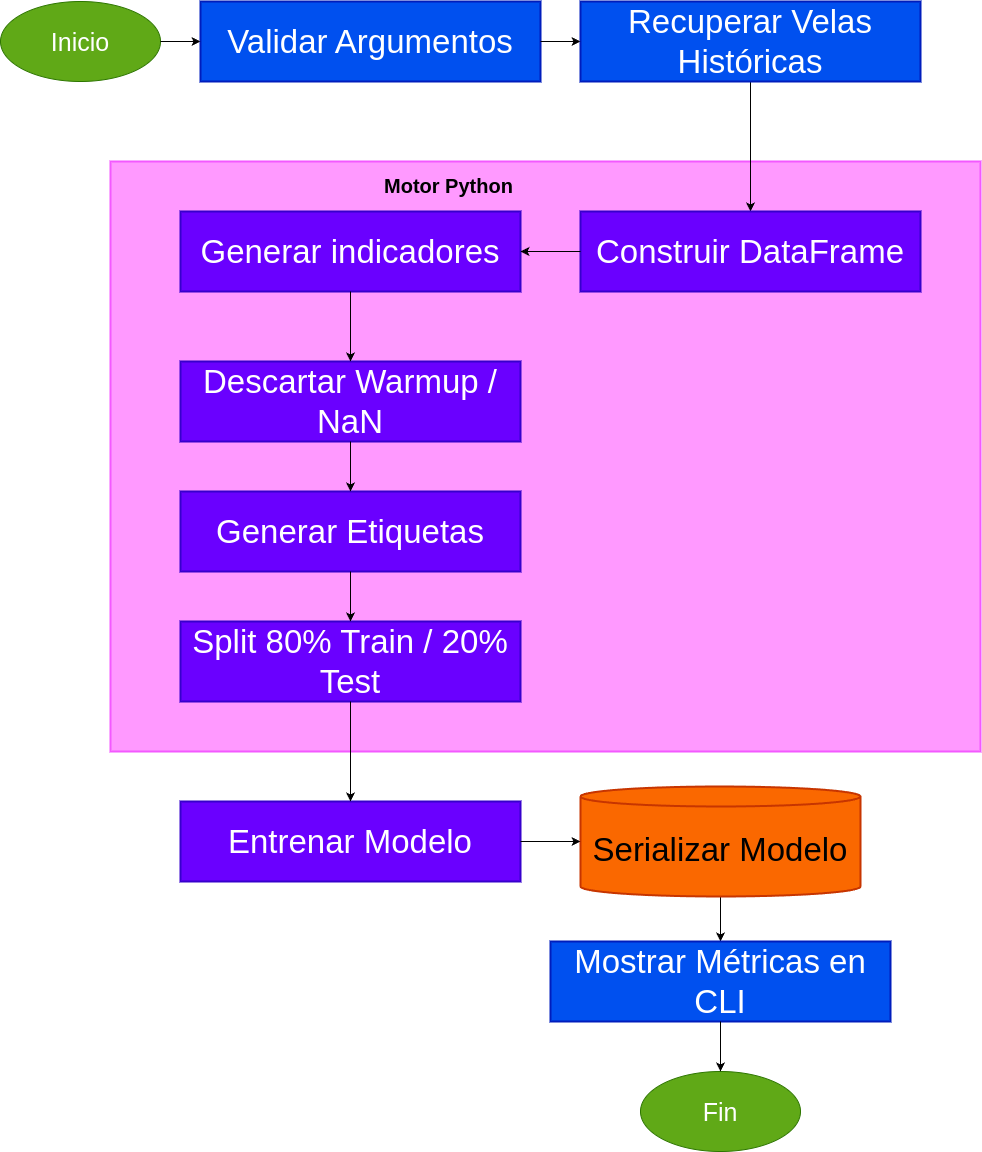
\includegraphics[width=0.7\linewidth]{Fotos/diagramas-flujo/train.png}
    \caption{Flujo de entrenamiento de modelos supervisados}
    \label{fig:train}
\end{figure}

% =============================================================================
\subsection{Optimización de Hiperparámetros}
% =============================================================================

La Figura~\ref{fig:optimize} ilustra el proceso de búsqueda automática de la
combinación óptima de hiperparámetros para un modelo dado, empleando Optuna
con el algoritmo \textit{Tree-structured Parzen Estimator} (TPE). Es la
operación más costosa computacionalmente del sistema: el servicio Java la
invoca con un \textit{timeout} de 3\,600 segundos, y el bucle de Optuna
ejecuta hasta 100 iteraciones (ensayos) por defecto, cada una de las cuales
incluye validación cruzada temporal y una simulación histórica real. Los
parámetros configurables desde la CLI son el tipo de modelo, el
\textit{timeframe}, el par de divisas, la estrategia Python, el umbral mínimo
de \textit{composite score} (por defecto 0,55), el número de ensayos
(\texttt{-n-trials}, por defecto 100) y el número de pliegues de validación
cruzada (\texttt{-cv-folds}, por defecto 5).

\textbf{Preparación del dataset con separación estricta.}
Antes de calcular ningún indicador, el motor divide el dataset en un 80\,\%
de entrenamiento y un 20\,\% de test respetando el orden cronológico. Esta
decisión es intencionada: separar primero y calcular indicadores después
sobre cada partición de forma independiente elimina cualquier riesgo de
filtración de información futura (\textit{data leakage}), incluso frente a
indicadores con componente global. Para que el conjunto de test disponga de
las velas de calentamiento que necesita la estrategia sin solaparse con el
de entrenamiento, el motor extiende la ventana de test hacia atrás
\texttt{get\_warmup\_period()} velas (\textit{lookback buffer}); esas filas
extra se eliminan después de calcular los indicadores, de forma que el
conjunto de test final comienza exactamente en el punto de corte 80/20.
Tras enriquecer ambas particiones con \texttt{populate\_indicators()}, se
descartan las filas del período de calentamiento y las que contengan valores
no finitos. Las etiquetas se generan a partir del umbral de retorno
\textit{forward-looking} de la estrategia (\texttt{LABEL\_RETURN\_THRESHOLD}),
produciendo tres clases: compra ($+1$), venta ($-1$) y neutro ($0$).

\textbf{Bucle de búsqueda Optuna.}
El estudio se crea con dirección de maximización y un podador
\texttt{MedianPruner(n\_startup\_trials=5, n\_warmup\_steps=10)}: los
primeros cinco ensayos nunca se podan para que el estimador de probabilidad
disponga de datos suficientes; a partir del sexto, Optuna interrumpe
anticipadamente cualquier ensayo cuya puntuación intermedia quede por debajo
de la mediana de los ensayos completados en el mismo paso. Esto reduce
significativamente el tiempo dedicado a regiones del espacio de búsqueda de
baja rentabilidad.

En cada ensayo, Optuna propone una combinación de hiperparámetros según el
espacio definido para el modelo seleccionado (véase el Anexo~\ref{anx:hiperparametros}
para el detalle de rangos). El motor evalúa esa combinación mediante
validación cruzada temporal con \texttt{TimeSeriesSplit}: en cada uno de los
$k$ pliegues, el conjunto de validación es siempre cronológicamente posterior
al de entrenamiento, lo que respeta la causalidad de las series temporales y
evita el sesgo de anticipación que introduciría un \textit{k-fold} clásico
aleatorizado. Para los modelos basados en \textit{scikit-learn} (XGBoost,
LightGBM, bosque aleatorio), el desbalance de clases se compensa asignando
pesos inversamente proporcionales a la frecuencia de cada clase mediante
\texttt{compute\_class\_weight("balanced")}. Para las redes neuronales,
estos pesos se pasan al método \texttt{fit()} de Keras y se añade
\texttt{EarlyStopping(patience=5)} sobre la pérdida de validación para
evitar sobreentrenamiento dentro de cada pliegue; además, durante la fase de
búsqueda, el motor limita el conjunto a las 50\,000 filas más recientes para
reducir el tiempo por ensayo, empleando el dataset completo únicamente en el
entrenamiento final.

Una vez completados todos los pliegues de un ensayo, el motor ejecuta una
simulación histórica real sobre el \textit{fold} más reciente (el que contiene
los datos cronológicamente más tardíos de entre todos los pliegues del
\texttt{TimeSeriesSplit}). Esta simulación utiliza las predicciones del modelo
entrenado en ese pliegue como señales de entrada y de salida para calcular las
métricas de trading que no se pueden derivar de la clasificación aislada:
tasa de acierto, factor de ganancia y ratio de Sharpe. La función de puntuación
compuesta integra entonces todas las dimensiones de calidad del ensayo:

$$\text{score} = 0{,}25 \cdot F1_{cv} + 0{,}40 \cdot \text{WinRate} + 0{,}25 \cdot PF_{norm} + 0{,}10 \cdot \text{Sharpe}_{norm} - \text{penalización}$$

donde $PF_{norm} = \min(\text{PF},\,5{,}0) / 5{,}0$ y $\text{Sharpe}_{norm} =
\max(0,\,\min(\text{Sharpe}/2{,}0,\,1{,}0))$ normalizan el factor de ganancia y
el ratio de Sharpe al intervalo $[0,\,1]$. La penalización se calcula como
$\max(0,\; (\text{acc\_train} - \text{acc\_cv}) - 0{,}05) \times 2{,}0$: solo
entra en juego cuando la brecha entre la exactitud sobre el conjunto de
entrenamiento y la exactitud en validación cruzada supera el 5\,\%, castigando
de forma progresiva los modelos que memorizan el conjunto de entrenamiento sin
generalizar.

El peso de 0,40 asignado a la tasa de acierto refleja una decisión de diseño
deliberada: en el contexto del trading simulado, que el modelo genere más
operaciones ganadoras que perdedoras tiene un impacto directo en la
rentabilidad final, más inmediato que la calidad de clasificación pura medida
por el F1. Por este motivo, la tasa de acierto domina la función objetivo por
encima del F1 (0,25), que penaliza los clasificadores que se especializan en
una sola clase a expensas del resto.

\textbf{Entrenamiento final y evaluación sobre el conjunto de test.}
Al terminar el bucle de Optuna, el motor identifica el ensayo con el
\textit{composite score} más alto, recupera su combinación de hiperparámetros
y entrena el modelo definitivo sobre el conjunto de entrenamiento completo
(el 80\,\% inicial). A continuación lo evalúa sobre el 20\,\% de test no
visto durante la búsqueda: calcula exactitud, precisión, recall y F1 mediante
las métricas de clasificación estándar y ejecuta una simulación histórica real
con las predicciones del modelo para obtener las métricas de trading finales
(tasa de acierto, factor de ganancia, caída máxima y ratio de Sharpe). El
modelo se serializa con Joblib en el directorio de modelos bajo un nombre
compuesto por tipo de modelo, estrategia, símbolo y \textit{timeframe}. Si
el \textit{composite score} del mejor ensayo no alcanza el umbral mínimo
configurado, el motor persiste igualmente el modelo, pero marca la respuesta
con estado \texttt{warning} en lugar de \texttt{success}. Todos los ensayos
completados y fallidos se guardan en un fichero CSV en el directorio de
resultados bajo el subdirectorio \texttt{optimize/}, con una fila por ensayo
que incluye todas las métricas intermedias y los hiperparámetros propuestos.

\textbf{Respuesta al orquestador Java.}
Python devuelve un \textit{envelope} IPC de tipo \texttt{OPTIMIZE\_RESPONSE}
que incluye: los hiperparámetros óptimos, el \textit{composite score} máximo
alcanzado y las métricas de clasificación y de trading del ensayo ganador, el
\textit{gap} de sobreajuste, la distribución de etiquetas del conjunto de
entrenamiento, el número de ensayos completados, las métricas finales sobre el
conjunto de test (tanto de clasificación como de simulación) y la ruta relativa
del CSV con el histórico de la búsqueda. Java imprime en consola un resumen
completo e informa al usuario si el umbral mínimo fue alcanzado o no.

\begin{figure}[H]
    \centering
    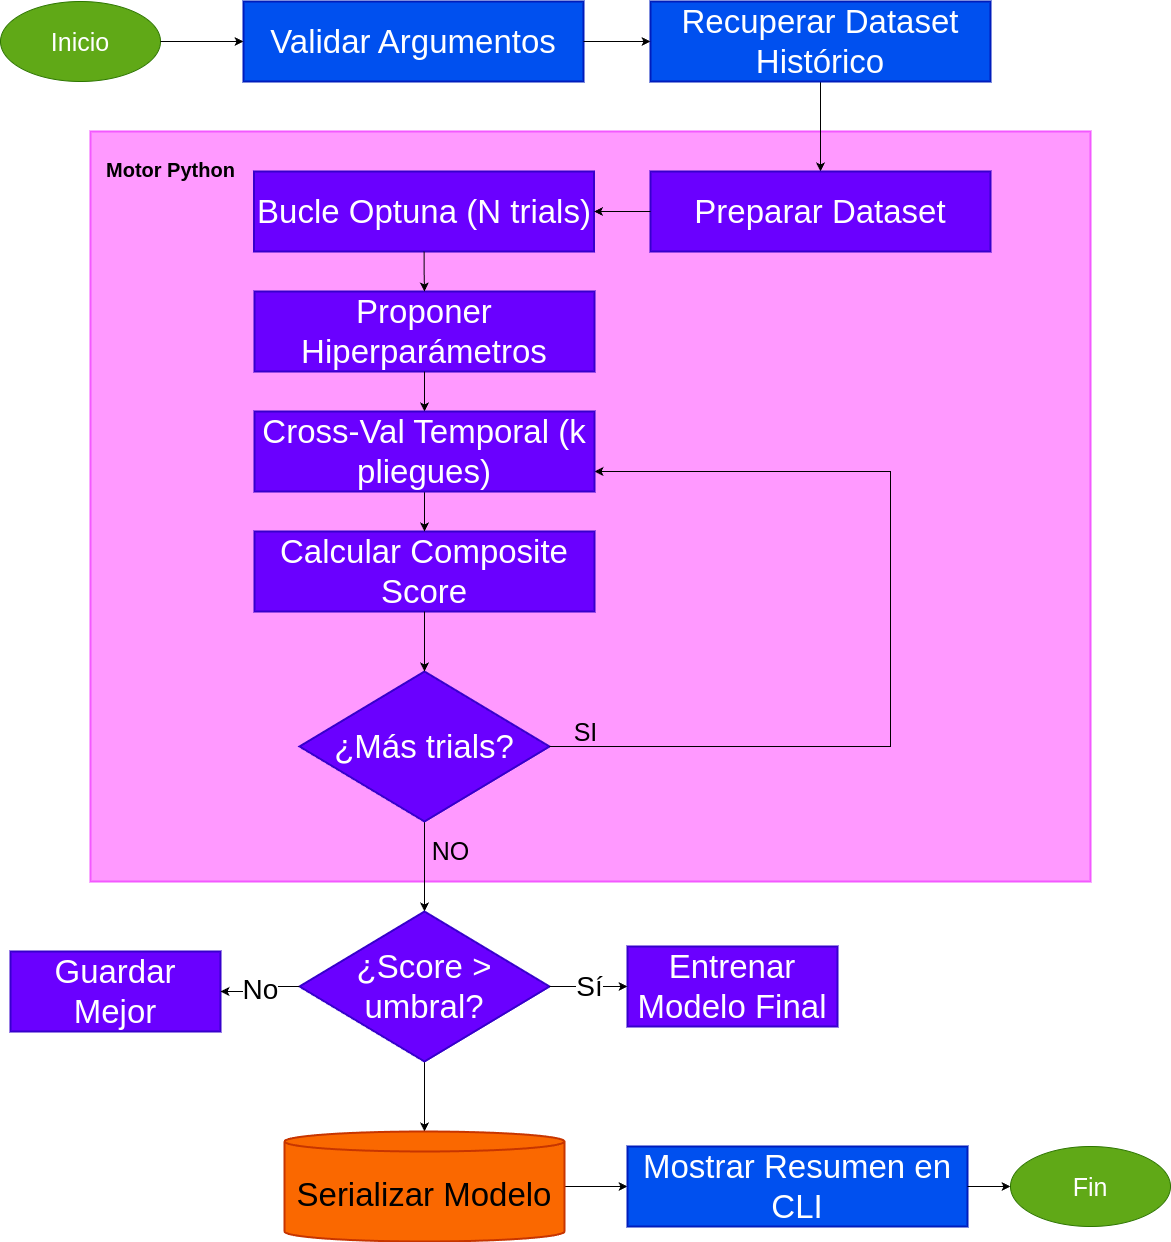
\includegraphics[width=0.7\linewidth]{Fotos/diagramas-flujo/optimize.png}
    \caption{Flujo de optimización de hiperparámetros}
    \label{fig:optimize}
\end{figure}

